\documentclass{standalone}

\usepackage{tikz}
\usepackage{amssymb}
\usetikzlibrary{calc, positioning}
\begin{document}
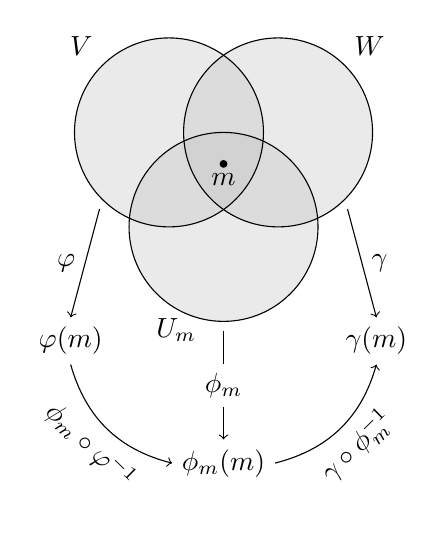
\begin{tikzpicture}
  \coordinate (m) at (0,0);

  \coordinate (v) at ($ (m) + (150:0.8) $);
  \node (v') at ($ (v) + (-135:1.2) $){};
  \coordinate (w) at ($ (m) + (30:0.8) $);
  \node (w') at ($ (w) + (-45:1.2) $){};
  \coordinate (u) at ($ (m) + (-90:0.8) $);
  \node (u') at ($ (u) + (-90:1.2) $){};

  \node[above left] at ($ (v) + (135:1.2) $){$ V $};
  \node[above right] at ($ (w) + (45:1.2) $){$ W $};
  \node[below] at ($ (u) + (-120:1.2) $){$ U_m $};

  \foreach \p in {(u), (v), (w)}{
    \fill[fill=gray!50, fill opacity=0.33] \p circle (1.2);
  }
  \foreach \p in {(u), (v), (w)}{
    \draw \p circle (1.2);
  }

  \draw[->] (v') to node[left]{$ \varphi $} ++(-0.4,-1.5) node[below] (v'') {$ \varphi(m)
    $};
  \draw[->] (w') to node[right]{$ \gamma $} ++(0.4,-1.5) node[below] (w'') {$ \gamma(m)
    $};
  \draw[->] (u') to node[fill=white]{$ \phi_m $} ++(0,-1.5) node[below] (u'')
    {$ \phi_m(m) $};

  \draw[->, bend right, sloped] (v''.south) to node[below]{$ \phi_m \circ \varphi
    ^{-1} $} (u''.west);
  \draw[->, bend right, sloped] (u''.east) to node[below]{$ \gamma \circ \phi_m
    ^{-1} $} (w''.south);

  \fill (m) circle (0.05) node[below]{$ m $};
\end{tikzpicture}
\end{document}
